\chapter{Bayesian regression models - probabilistic surrogate model}
As mentioned in the previous sections, the first of two repeated steps in Bayesian optimization
is to create a good Bayesian regression model. %why not non bayesian regression? 
i.e. finding the probility of prediction for a arbitrary point $x$ given datapoints 
$\mathcal{D} = \{x_1, y_1, \dots, x_n, y_n\}$, 
 $$p(y|x,\mathcal{D})$$

The surrogate model of choise in Bayesian optimization is a Gaussian Process, and Bayesian Neural Network.
These are discriminative models, however, another approach, which we focus on in this project, is
to model $y$ and $x$ jointly in a so-called generative model.

\section{Gaussian mixture regression}
Taking a convex combination of a set of multivariate Gaussian distributions is a Gaussian mixture model
$$p(z) = \sum_{k=1}^K \pi_k \mathcal{N}(z|\mu_k, \Sigma_k)$$  
Defining $z := (x,y)$ we can model our data, as a generative model $p(x,y)$, now, since the conditonal 
of a Gaussain mixture again is Gaussain mixture - i.e. closed form expression, we can exactly calculate
$p(y|x) = GMM_{y|x}$

Assuming iid data the likelihood is given as 
$$p(\mathcal{D}|\mu_1, \dots, \mu_K, \Sigma_1, \dots, \Sigma_K, \pi_1, \dots, \pi_K) = \prod_{i=1}^n \sum_{k=1}^K \pi_k \mathcal{N}(z_i|\mu_k, \Sigma_k)$$
And the log likelihood, 
$$\log p(\mathcal{D}| ..) = \sum_{i=1}^n \log \sum_{k=1}^K \pi_k \mathcal{N}(z_i|\mu_k, \Sigma_k)$$


\section{Mixture regression in a Bayesian setting}
As seen in examples. The uncertainty of conditional distribution is way too certain
in areas with no data points, therefore we need to enhance the model with some bayesian 
flavour. 

$$p(y|x,\mathcal{D}) = p(y|x,Z)p(Z|x)$$



\subsection*{Expetation-maximization algorithm}
A way to find local maxima in the likehood function is using the EM algorithm. 

If we define a latent/hiddem random variabel $Z_i \in \{1,\dots, K\}$ for each data point, then 
the likelihood function becomes, 
$$L(\theta|\mathcal{D}, Z) = \prod_{i=1}^n \sum_{k=1}^K 1(Z_i = k) \pi_k \mathcal{N}(z_i|\mu_k, \Sigma_k)$$

Now the expectation wrt. the current value $p(Z|\mathcal{D}, \theta^k)$ is given as 
$$Q(\theta|\theta^k) = \mathcal{E}_{p(Z|\mathcal{D}, \theta^k)}=L(\theta|\mathcal{D}, Z) $$

And then update the next parameter estimate with
$$\theta^{k+1} = \arg \max_{\theta} Q(\theta|\theta^k)$$

This is repeated untill convergence. 


\section{Sum product networks}
We will for a large extend just see SPN as a large mixture model. This is a totally valid observation. 

\subsection*{Mixture model}
%from [@desana]:
\begin{definition} 
    A sub-network $\bar S_z$ of $S$ is an SPN, which includes the root $S$ and then includes nodes
    according to the following recursive scheme: 
\end{definition}
\begin{algorithm}[H]
    \caption*{Collection of sub-network $S_z$ of $S$}\label{SPN4}
    \begin{algorithmic}
    %\State \textbf{Global:}  $S_z$ 
    \Function{Process}{node i, $S_z$}
    \If{$i \in \mathcal{L}eaf(S)$}
        \State  $\textbf{return: }$ 
    \EndIf
    %\For{$i \in I_{o}$}
    \If{$i\in \mathcal{S}um(S)$}
       %\State $S_z =S_z \cup \{j \in ch(i)\}$ \Comment{include one child of node $i$}
        \State $S_z =S_z.add(j \in ch(i))$ \Comment{include one child of node $i$}
        \State $\textbf{return: } \text{Process}(j, S_z)$
    \EndIf
    \If{$i\in \mathcal{P}rod(S)$}
        \State $S_z =S_z \cup \{j | j \in ch(i)\}$ \Comment{include all childen of node $i$}
        \For{$j \in ch(i)$}
            \State $\textbf{return: } \text{Process}(j,S_z)$
        \EndFor
    \EndIf
    \State $\textbf{return: } S_z$
    \EndFunction
    \State $S_z =  \text{Process(root,Ø)}$
    \end{algorithmic}
\end{algorithm}
So we see that at each sum node the number of different sub-networks multiplies with the number of children for that
sum node. And thereby, the total number of sub-networks is
 $$Z = \prod_{i\in \mathcal{S}um(S)}|ch(i)|$$ 
 i.e. an exponential large amount of sub-networks. This is the amount of
 mixture components implicitly defined in an SPN. 
 Denote the set of edges in the sub-network $\mathcal{E}(S_z)$.
Now the we define a mixture coeficient, $\lambda_z$ and component for each $S_z$ as 
$$\lambda_z := \prod_{(i,j)\in \mathcal{E}(S_z)} w_{i,j}, \hspace{1cm}
p_z(x,y|\theta) := \prod_{i \in \mathcal{L}(S_z)} p_i(x,y)$$
where $p_i(x,y)$ is the leaf distribution at leaf node $i$ paramitised with $\theta$. 
It can now be proven that the SPN can be interpreted as the following mixture model, 
$$p(x,y|w,\theta) = \sum_{z=1}^Z \lambda_z(w)p_z(x,y|\theta)$$
i.e. by the weighted sum of all $Z$ sub-networks. For convinience
we define each sum component as $p(z,x,y|w,\theta) := \lambda_z(w)p_z(x,y|\theta)$.
Evaluation of $p(x,y|w,\theta)$ will never be done as the sum over $Z$ components, 
instead there is a proposition. 

\begin{proposition}
    Consider a SPN, S, a sum node $q \in \mathcal{S}um(S)$ and a child $i \in ch(q)$,
    then the following relation holds, 
    $$\sum_{z:(q,i)\in \mathcal{E}(S_z)} \lambda_z(w) p_z(x,y|\theta) = w_{i,q}
    \frac{\partial S}{\partial v(q)} v(i)$$
\end{proposition}



\subsection*{Conditional of SPN}

We will soon see how it is possible to write the conditional distribution as the mixture, 
$$p(y|x) = \sum_{z \in \Sigma(S)} \gamma(x) p_{z_y}(y)$$
where $ \Sigma(S)$ is the set of all sub-networks in the SPN, $S$ - \todo{IT IS EXPONENTIALLY LARGE}.  
And where $p_{z_y}(y)$ is defined through $p_z(x,y)$, 
\begin{align*}
    p_z(x,y) &= \prod_{l \in \mathcal{L}eaf(z_x)} \phi_l(x)\prod_{l \in \mathcal{L}eaf(z_y)} \phi_l(y)\\
            &=: p_{z_x}(x) p_{z_y}(y) 
\end{align*}
where $\phi_l$ is the density of the $l$'th leafs tractable distribution. Recall that we can interpret an SPN
as the mixture model, 
$$p(x,y) = \sum_{z \in \Sigma(S)} \lambda_z p_z(x,y)$$
where $\lambda_z = \prod_{(q,j) \in \mathcal{E}(z)} w_{q,j}$. First we calculate the marginal density,
$p(x)$, 
\begin{align*}
    p(x) &= \int p(x,y)dy\\
    &= \int \sum_{z \in \Sigma(S)} \lambda_z p_z(x,y)dy\\
    %&= \sum_{z \in \Sigma(S)} \lambda_z  \int p_z(x,y)dy\\
    &= \sum_{z \in \Sigma(S)} \lambda_z p_{z_x}(x)\int p_{z_y}(y)dy \\
    &= \sum_{z \in \Sigma(S)} \lambda_z p_{z_x}(x)
\end{align*}
Now we are ready to calculate the conditional density, 
\begin{align*}
    p(y|x) &=  \frac{p(x,y)}{p(x)}\\
            &= \frac{\sum_{z \in \Sigma(S)} \lambda_z p_z(x,y)}{p(x)}\\
            &=\sum_{z \in \Sigma(S)}\frac{ \lambda_z p_{z_x}(x)}{p(x)} p_{z_y}(y)\\
            &=\sum_{z \in \Sigma(S)}\frac{ \lambda_z p_{z_x}(x)}{\sum_{z \in \Sigma(S)} \lambda_z p_{z_x}(x)} p_{z_y}(y)\\
            &=\sum_{z \in \Sigma(S)} \gamma(x) p_{z_y}(y)
\end{align*}
So we defined $\gamma(x) = \frac{ \lambda_z p_{z_x}(x)}{\sum_{z \in \Sigma(S)} \lambda_z p_{z_x}(x)}$ 
and this is very convinient, as we will see soon is 
equavalent to the derivative of the log-likehood
of the SPN, which is easily obtained by automatic differentiation. 

\subsection*{calculation of $\gamma(x)$}
expectation maximization of a mixture model, is given by Bishop..
the responsibility of a datapoint to belong to one mixture component, is given by
$$\gamma(z_{nk}) = \frac{w_k p_j(x_n)}{\sum_i w_i p_i(x_n)}$$
We can prove that the responsibility is equal to the gradient of the log likehood, 
$$L:= \sum_n \log \sum_j w_j \exp \psi_j(x_n)$$
where we define $\psi_j(x_n) = \log p_j(x_n)$. Take the gradient 
$$\frac{\partial L}{\partial \psi_{j}(x_{n})} = \frac{w_k p_j(x_n)}{\sum_i w_i p_i(x_n)}$$
Note that the gradient easily can be found using autograd. 


\subsection*{Mean and variance of $p(y|x)$}

The mean of the conditional is just
\begin{align*}
    E_{p(y|x)}[y] &= \sum_{z \in \Sigma(S)} \gamma(x) \int  y p_{z_y}(y) dy \\
    &= \sum_{z \in \Sigma(S)} \gamma(x) \prod_{l \in \mathcal{L}eaf(z_y)} E_{\phi_l}[y]
\end{align*}

and the variance is found using the second moment, 
\begin{align*}
    E_{p(y|x)}[y^2] &= \sum_{z \in \Sigma(S)} \gamma(x) \int  y^2 p_{z_y}(y) dy \\
    &= \sum_{z \in \Sigma(S)} \gamma(x) \prod_{l \in \mathcal{L}eaf(z_y)} (Var_{\phi_l}[y]+E_{\phi_l}[y]^2)
\end{align*}



SPN is an exponential large mixture model, with linear inference - unlike GMM. !?
\todo{Write naive bayesian mixture model as a Sum Product Network}

sum nodes play a role of
mixtures over their children distribution, similar to a classic mixture model

Product
nodes on the other hand, are equivalent to factorizations over independent distributions as they are
combining disjoint RVs.

SPNs can also be interpreted as deep feed forward neural network [@vergari]. Here, imagine the
weights of the sum nodes are parameters, leaf distributions are input neurons, root node is output and
all other nodes correspond to hidden neurons


\begin{figure}[H]%
    \centering
    {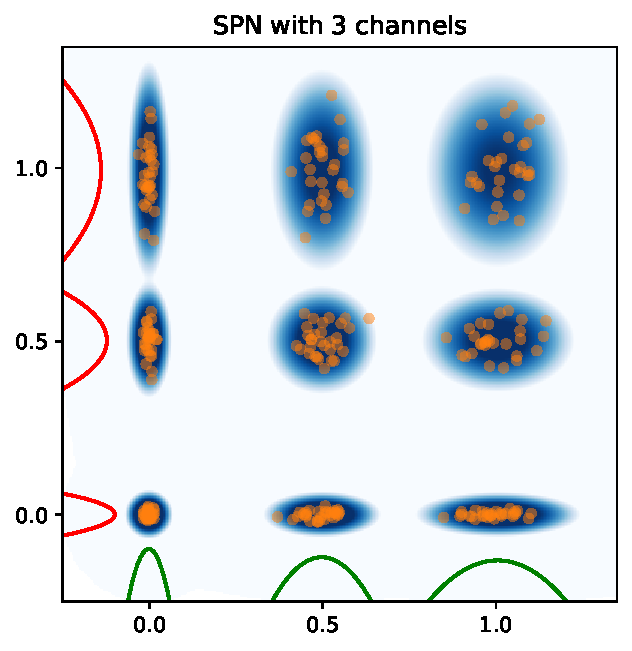
\includegraphics[width=0.46\textwidth]{Pictures/SPN_illustration1.pdf} }%
    \qquad
   {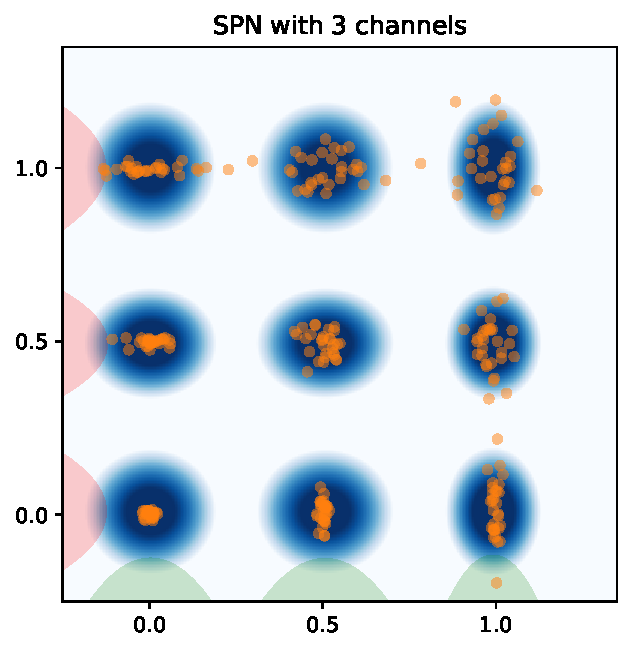
\includegraphics[width=0.46\textwidth]{Pictures/SPN_illustration2.pdf} }%
    \caption{SPN}%
    \label{SPN_fig}%
\end{figure}

\begin{figure}[htbp]
    \centering
    \begin{tikzpicture}

  % Define nodes

   % Define nodes
   \node[latent] (x4) {${x}_4$};
   \node[latent, left=of x4] (x3) {${x}_3$};
   \node[latent, left=of x3] (x2) {${x}_2$};
    \node[latent, left=of x2] (x1) {${x}_1$};
    \node[latent, left=of x1] (x0) {${x}_{0}$};
    
    \node[latent, below=of x4] (x4_hat){$\hat{{x}}_4$};
    \node[obs, below=of x3] (x3_hat){$\hat{{x}}_3$};
    \node[latent, below=of x2] (x2_hat){$\hat{{x}}_2$};
    \node[latent, below=of x1] (x1_hat){$\hat{{x}}_1$};
    \node[obs, below=of x0] (x0_hat){$\hat{{x}}_0$};
    
    \node[const, below= of x2_hat] (sigma-eps) {$\sigma_\epsilon$};
    \node[const, above= of x2] (sigma) {$\sigma$};

%   % Connect the nodes
%    \edge {I-0} {wifi-strength};
    \edge {x1} {x1_hat} ; %
    \edge {x0} {x0_hat} ;
    \edge {x2} {x2_hat} ; %
    \edge {x3} {x3_hat} ;
    \edge {x4} {x4_hat} ; %
    % \edge {a} {sensor-data} ; %

  \edge {x0} {x1} ; %
  \edge {x1} {x2} ; %
  \edge {x2} {x3} ; %
  \edge {x3} {x4} ; %
  
  \edge {sigma} {x1} ; %
  \edge {sigma} {x0}
    \edge {sigma} {x2} ; %
  \edge {sigma} {x3}
    \edge {sigma} {x4} ; %

  \edge {sigma-eps} {x1_hat} ; %
  \edge {sigma-eps} {x0_hat}
   \edge {sigma-eps} {x2_hat} ; %
  \edge {sigma-eps} {x3_hat}
   \edge {sigma-eps} {x4_hat} ; %
%    \plate{} {(wifi-location)(wifi-strength)(wifi-sensor)} {$K$}
%    \plate{} {(x)(x_)(wifi-sensor)(x_hat)} {$T$}
%    \plate{} {(x1)(x0)(x1_hat)} {$T$}    

%   % Plates
%   \plate {yx} {(x)(y)} {$N$} ;
%   \plate {} {(w)(y)(yx.north west)(yx.south west)} {$M$} ;
\end{tikzpicture}
    \caption{Model including wifi information}
    \label{fig:wifi2}
\end{figure}

\begin{figure}[H]
    \centering
    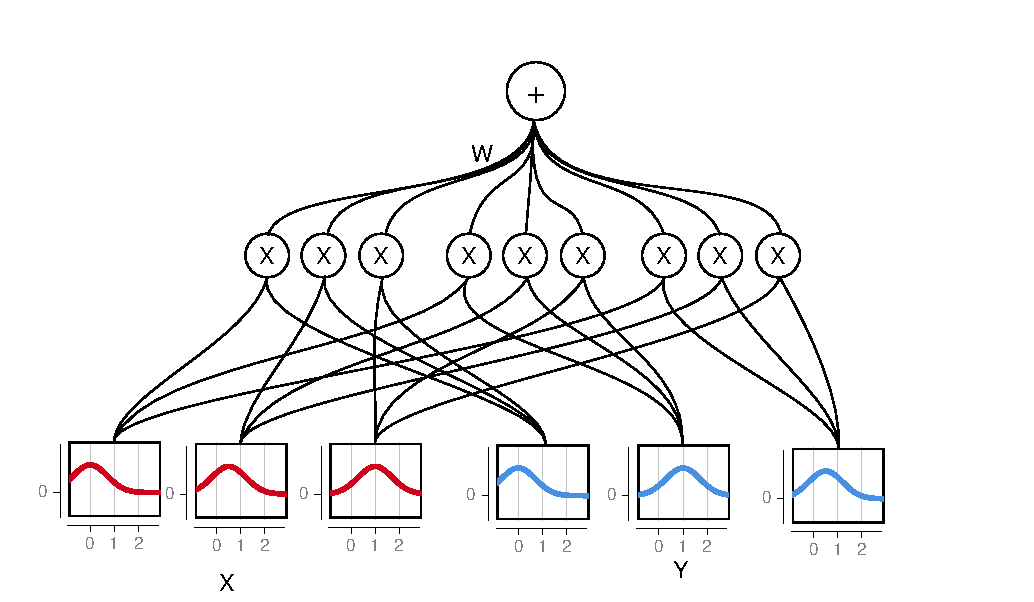
\includegraphics[width=\textwidth]{Figures/SPN_graph2.pdf}
\end{figure}